% Results. Every number is a macro from generated_numbers.tex (experiments/paper_figures.py).
\section{Results}
\subsection{Protocol}
All allocations, scheme choices and truncation depths are selected on 5,000 validation images with three
channel seeds. The test split (10,000 images, five channel seeds) is used once for the final numbers. Gains
are paired against uniform RS under identical loss realizations. We report 95\% intervals over channel
seeds and, for gains, a bootstrap over test images. The exact simulator reproduces the published
RS-decoded sweep of the primary model to within \ReferenceMaxDiff~dB on \ReferenceCells{} overlapping
cells. Unless stated otherwise, results are for the primary ADJSCC-Q model (clean test PSNR
\CleanPsnr~dB). The LOO ranking is a single static table per checkpoint, measured on the training split,
so it costs no side information.

\subsection{Erasure sensitivity is concentrated and attention does not see it}
Fig.~\ref{fig:profiles} shows the sorted share of LOO MSE damage per channel. The four most damaging channels
carry \TopFourShareMinAdj--\TopFourShareMaxAdj\% of it in ADJSCC-Q (\SeedsAdj{} converged seeds) and
\TopFourShareMinDeep--\TopFourShareMaxDeep\% in DeepJSCC-Q (\SeedsDeep{} converged seeds, same GPU type).
The concentration is therefore not created by the attention modules. Profiles agree across seeds, but
channel indices permute, so a ranking belongs to a checkpoint. On 2,000 validation images the
within-image Spearman correlation between the bottleneck attention gate and true damage is $-0.015$ (top-4
overlap 0.23 against 0.25 by chance). Latent energy reaches $+0.84$, and a two-layer head with 2,048 MACs
(0.04\% of the encoder) reaches top-4 overlap 0.92. The CIFAR-10 ranking transfers to CIFAR-100 with
Spearman 0.997.

\begin{figure}[t]\centering
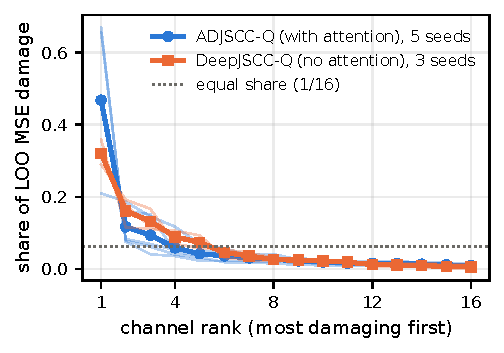
\includegraphics[width=\columnwidth]{figures/fig_profiles.pdf}
\caption{Sorted share of leave-one-out MSE damage per latent channel (thin: individual seeds; thick:
mean). Both architectures concentrate damage far above the equal share.}
\label{fig:profiles}
\end{figure}

\subsection{Where does tiered UEP gain come from?}
At 40\% loss uniform RS(96,64) fails in most images (\UniformForty~dB). The hand-designed 25/50/25 scheme
gains \HandTierGainForty~dB with the static LOO order, \HandTierAttentionGainForty~dB with attention and
\HandTierRandomGainForty~dB with a random order. A per-image LOO order (an unattainable upper bound) gains
\HandTierPerImageGainForty~dB. The unsorted two-tier control (two RS(48,32) blocks at the uniform rate)
isolates block length: \TwoTierUnsortedGainForty~dB at 40\% and \TwoTierUnsortedGainThirty~dB at 30\%. The
PET twin of the 25/50/25 scheme gains \PetTwinGainForty~dB, so sharing packets across tiers does not
rescue the hand-designed allocation. Below about 32\% loss the fixed scheme falls
behind uniform RS (\HandTierGainTwenty~dB at 20\%) because its bottom tier carries no parity.

\subsection{The optimal allocation is importance-ordered truncation}
Fig.~\ref{fig:main} and Table~\ref{tab:alloc} report the validation-optimized designs. Up to 20\% loss the
search returns uniform RS. From 30\% on it returns truncation (the top \TruncKeepThirty, \TruncKeepForty{}
and \TruncKeepFifty{} channels for 30, 40 and 50\% loss, each in one RS($96,4m$) block), or a PET or
three-level layout within a few tenths of a dB of it. Simulating the 25 surrogate-best genuinely multi-tier allocations improves on
truncation by at most \MultiTierMaxGain~dB on validation. PET designs are within \PetVsTruncMax~dB. On the
test split, truncation in LOO order gains \TruncOracleGainForty~dB at 40\% loss and
\TruncOracleGainFifty~dB at 50\%, about \TruncOverHandForty~dB more than the hand-designed scheme. It is
never worse than uniform RS at low loss, because there the selected design \emph{is} uniform RS.

The ranking now decides almost everything. With the same validation-chosen depth, truncation in random
order gains only \TruncRandomGainForty~dB at 40\% loss, in attention order \TruncAttentionGainForty~dB,
in energy order \TruncEnergyGainForty~dB, and with the 2,048-MAC head \TruncHeadGainForty~dB.
Proposition~\ref{prop:trunc} explains why: the coding gain of truncation is paid for by the damage of the
channels left out, which only an accurate ranking keeps small. The additive surrogate~\eqref{eq:surrogate}
predicts the simulated mean MSE of the test-evaluated layouts with Spearman correlation
\SurrogateSpearman{} and median relative error \SurrogateMedianRelErr\% (Fig.~\ref{fig:surrogate}), so the
allocation can be designed in closed form. The surrogate underestimates the MSE when many channels are
partially lost at once, because damage is mildly superadditive. It still ranks layouts well, and the final
choice is always made by exact simulation.

\begin{figure}[t]\centering
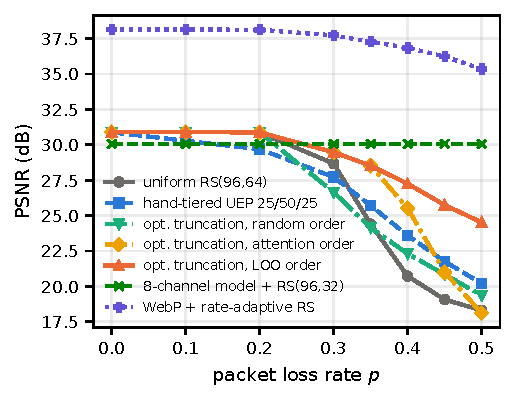
\includegraphics[width=\columnwidth]{figures/fig_main.pdf}
\caption{Test PSNR versus packet loss rate (1,536 transmitted bytes per image). Optimized allocations are
chosen per loss rate on validation. All curves except the 8-channel, ordered and WebP ones use the
primary model.}
\label{fig:main}
\end{figure}

\begin{table}[t]\centering\caption{Test PSNR (dB) and gain over uniform RS at 40\% loss}\label{tab:alloc}
\begin{tabular}{lrr}\toprule
Method & PSNR & gain\\\midrule
uniform RS(96,64) & \UniformForty & --\\
no RS (64 packets, 32 idle) & \NoRSForty & \NoRSGainForty\\
hand-tiered 25/50/25, LOO order & \HandTierForty & \HandTierGainForty\\
PET twin of 25/50/25 & \PetTwinForty & \PetTwinGainForty\\
Grad-FEC style (top 8 coded, 4 dropped) & \GradFecForty & \GradFecGainForty\\
opt.\ truncation, random order & \TruncRandomForty & \TruncRandomGainForty\\
opt.\ truncation, attention order & \TruncAttentionForty & \TruncAttentionGainForty\\
opt.\ truncation, energy order & \TruncEnergyForty & \TruncEnergyGainForty\\
opt.\ truncation, 2,048-MAC head & \TruncHeadForty & \TruncHeadGainForty\\
opt.\ truncation, LOO order & \TruncOracleForty & \TruncOracleGainForty\\
opt.\ grouped (multi-tier allowed) & \OptGroupedForty & \OptGroupedGainForty\\
opt.\ PET & \OptPetForty & \OptPetGainForty\\\bottomrule
\end{tabular}\end{table}

\begin{figure}[t]\centering
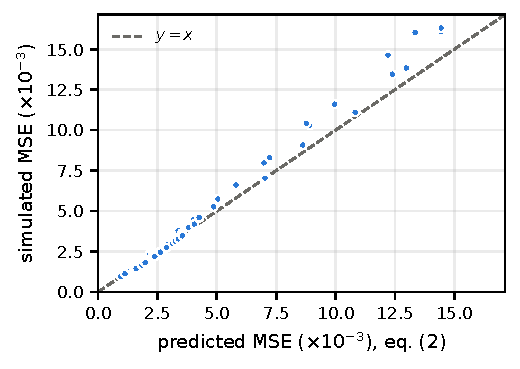
\includegraphics[width=\columnwidth]{figures/fig_surrogate.pdf}
\caption{Additive surrogate~\eqref{eq:surrogate} versus simulated mean MSE for every LOO-ordered layout and
loss rate evaluated on the test split.}
\label{fig:surrogate}
\end{figure}

\subsection{Unknown loss rate}
A design is only optimal at the loss rate it was made for. Fig.~\ref{fig:mismatch} shows the cost of
mismatch. A truncation designed for 40\% loss gives up \DesignFortyAtZeroLoss~dB on a clean channel and
gains \DesignFortyAtFifty~dB at 50\%. A single allocation optimized over $p\in[0.1,0.5]$ changes the PSNR by
\RobustGroupedGainForty~dB at 40\% and by \RobustGroupedGainTen~dB at 10\%. This is the only regime in which
the search selects a multi-level structure (the robust PET design: \RobustPetGainTen~dB at 10\%,
\RobustPetGainForty~dB at 40\%). With loss-rate feedback, the selector of Table~\ref{tab:alloc} (one byte
of signalling per loss-rate change) is the operating point we recommend.

\begin{figure}[t]\centering
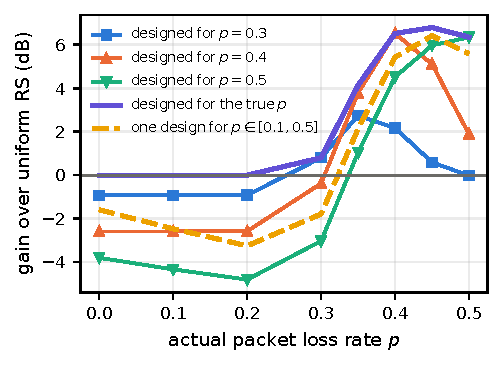
\includegraphics[width=\columnwidth]{figures/fig_mismatch.pdf}
\caption{Gain over uniform RS of allocations designed for one loss rate and used at another.}
\label{fig:mismatch}
\end{figure}

\subsection{Baselines that change the picture}
\emph{Smaller models.} Truncating a 16-channel model to $m$ channels competes with a model trained for
$m$ channels. With the same 96 packets, the 8-channel model (bandwidth ratio 1/12) behind RS(96,32) gives
\KnTwelveClean~dB at every loss rate up to 50\%: its code essentially never fails, and halving the latent
costs only about 0.8~dB of clean quality. The 6-channel model
behind RS(96,24) gives \KnSixteenForty~dB. Switching between such models dominates truncating an
unordered model at high loss. Truncation is the single-model approximation to this envelope, and its
quality is set by the ranking.

\emph{Ordered latents.} Nested (tail) dropout \cite{rippel2014nested} closes this gap with one network. During
training, half of the images keep only a uniformly random prefix of the 16 channels. The resulting LOO order
equals the channel index, and the clean cost is \OrderedCleanCost~dB. Truncation in index order then barely
depends on the loss rate: \OrderedTruncForty~dB at 40\% and \OrderedTruncFifty~dB at 50\% loss. On the same
model, uniform RS gives \OrderedUniformForty~dB and truncation in random order \OrderedRandomForty~dB at
40\%. The ordered model is above the 8-channel model at every loss rate. The DeepJSCC-Q counterpart
behaves the same (\OrderedDeepTruncForty~dB at 40\%, \OrderedDeepClean~dB clean). In the ordered ADJSCC-Q
model the last five channels carry almost nothing (each LOO drop at most 0.02~dB). Nested dropout thus
trades unused capacity for an embedded order, which is exactly what classical ULP assumes.

\emph{No RS at all.} A 24-channel model can spend all 1,536 bytes on latent symbols and be fine-tuned
over packet erasures, so that it degrades gracefully without any code. None of three 24-channel ADJSCC-Q
runs converged under our recipe (best clean validation PSNR \NoRsBestValClean~dB, below the 16-channel
model). The DeepJSCC-Q recipe did converge, so we compare within it.
\begin{itemize}
\item \emph{No RS, 24 channels, erasure fine-tuned:} \NoRsDeepForty~dB at 40\% loss (\NoRsDeepClean~dB clean).
\item \emph{RS with LOO truncation, 16 channels:} \RsDeepTruncForty~dB at 40\% (\RsDeepClean~dB clean).
\item \emph{The same, after the same fine-tuning:} \RsDeepRobustTruncForty~dB at 40\%.
\end{itemize}
Without RS the quality falls from the first lost packet (\NoRsDeepThirty~dB at 30\%, against
\RsDeepTruncThirty~dB). Packet-level RS with truncation is therefore the better use of the budget up to
45\% loss. At 50\%, the fine-tuned no-RS model (\NoRsDeepFifty~dB) passes truncation of the plain model
(\RsDeepTruncFifty~dB) but not of the fine-tuned one (\RsDeepRobustTruncFifty~dB).

\emph{Conventional codecs.} Earlier comparisons in this line gave JPEG, JPEG2000 and WebP a fixed
RS(96,64) code, which collapses beyond 33\% loss (WebP: \WebpFixedForty~dB at 40\%). Allowed the same
choice we give the JSCC transmitter, i.e.\ fewer source bytes and a stronger code chosen on validation, WebP
keeps \WebpAdaptiveForty~dB at 40\% and \WebpAdaptiveFifty~dB at 50\% loss, above every JSCC system
here (clean: \WebpAdaptiveZero~dB versus \CleanPsnr~dB). At this rate, byte-quantized JSCC without entropy
coding is far from codec efficiency. Our conclusions are about how to protect a learned latent once it
is the transmitted representation, not about JSCC versus separation.

\subsection{Across model seeds and architectures}
Table~\ref{tab:seeds} repeats the main comparison for every converged model, each with its own LOO
ranking and validation-chosen truncation depth. LOO-ordered truncation gains \TruncGainMinAdj{} to
\TruncGainMaxAdj~dB over uniform RS at 40\% loss for ADJSCC-Q and \TruncGainMinDeep{} to
\TruncGainMaxDeep~dB for DeepJSCC-Q, and beats the hand-tiered scheme on every model
(\TruncOverHandMinAll{} to \TruncOverHandMaxAll~dB). The primary model is the most favourable ADJSCC-Q
seed. Energy order is within 0.9~dB of LOO order on every model, while attention order is unreliable:
it ranges from below the random order (ADJSCC-Q seed 21) to 1.5~dB under LOO order.
\begin{table}[t]\centering\caption{Test PSNR (dB) at 40\% loss across models}\label{tab:seeds}
\resizebox{\columnwidth}{!}{% generated by experiments/paper_figures.py -- do not edit
\begin{tabular}{lrrrrrrr}
\toprule
model & clean & uniform & hand-tiered & \multicolumn{4}{c}{opt.\ truncation, order:} \\
 & & & LOO & LOO & energy & attention & random \\
\midrule
ADJSCC-Q s100 & 31.34 & 20.77 & 23.60 & 25.77 & 25.75 & 23.15 & 22.28 \\
ADJSCC-Q s13 & 31.76 & 20.64 & 23.54 & 26.18 & 26.36 & 22.41 & 22.13 \\
ADJSCC-Q s21 & 31.09 & 20.79 & 23.90 & 26.14 & 25.27 & 20.78 & 22.24 \\
ADJSCC-Q s42 & 30.88 & 20.73 & 23.59 & 27.25 & 26.72 & 25.72 & 22.42 \\
ADJSCC-Q s7 & 31.45 & 21.02 & 23.37 & 25.04 & 25.74 & 23.25 & 22.70 \\
DeepJSCC-Q s100 & 31.79 & 18.56 & 22.19 & 28.00 & 27.89 & -- & 20.54 \\
DeepJSCC-Q s21 & 32.73 & 19.52 & 22.70 & 25.63 & 26.03 & -- & 21.51 \\
DeepJSCC-Q s7 & 32.17 & 17.81 & 21.86 & 26.03 & 26.08 & -- & 19.64 \\
\bottomrule
\end{tabular}
}
\end{table}

\section{Discussion and Limitations}
The study uses $32{\times}32$ images, one bandwidth ratio for the primary analysis, i.i.d.\ losses for the
allocation results, and a known loss rate for the selector. Under Gilbert--Elliott bursts with 45\% average
loss, LOO truncation still beats uniform RS, by \BurstTruncGainOne~dB with i.i.d.\ losses and by
\BurstTruncGainSixteen~dB at a mean burst length of 16 packets. The interleaved hand-tiered scheme gains
\BurstHandGainOne~dB and \BurstHandGainSixteen~dB respectively. Choosing the truncation depth for the burst
statistics adds at most \BurstDepthGainMax~dB. The SSIM implementation of the code base uses zero-padded
windows, so we report PSNR only. Two of five DeepJSCC-Q seeds and one of six ADJSCC-Q seeds did not
converge under the common recipe; they are excluded by a rule fixed before evaluation.
